\section{Introduction}

Our world is full of things that move.
Increasingly, because of sensors like GPS, we have data of where things are and when they were there.
This data is useful for revealing properties of the thing's movement: like \emph{how fast did it move?} or \emph{how far did it travel?}
Further, this data can be used to describe aggregate properties of many things, like how many cars drive on the road by my house?
This kind of analysis has been very fruitful because it allows us to understand something about what happened.

\begin{wrapfigure}{l}{0.33\textwidth}
  \centering
  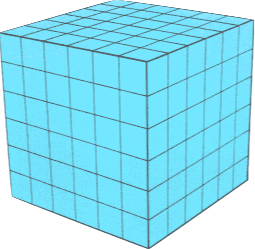
\includegraphics[width=0.32\textwidth]{./figures/unitCube}
  \caption{Unit cube space used in spatial abstraction.}
  \label{fig:unitCubes}
\end{wrapfigure}

However, analyzing this data can be hard because there are an overwhelming number of data points.
Also is can be very difficult to examine higher-level relationships because points and lines are overly specific.  
Often it is only feasible to analyze large data sets by choosing an appropriate level of abstraction.
This work is about one such kind of abstraction, a spatial abstraction where particular points in space-time are mapped to unit cubes, as shown in Fig.~\ref{fig:unitCubes}.
Using techniques inspired by software analysis, specifically Daikon invariants~\cite{kataoka2001automated}, we explore the properties of movement of things at a higher level, and the relationships between these properties.

We explore what properties exist within this abstraction and how these properties can be used to reason about how one or more things moved in time.

This paper is organized as follows:
1) Section~\ref{sec:background} gives an overview of both spatial analysis and the Daikon invariants analysis tool;
2) Section~\ref{sec:method} describes the method of spatial abstraction, including defining terms and a table of formalized properties;
3) Section~\ref{sec:tool} provides an overview of our tool that implements this method of analysis;
4) Section~\ref{sec:experiments} shows an initial application of our tool to a real robotic system;
5) Section~\ref{sec:related} situates this work relative to other kinds of movement analysis;
6) Section~\ref{sec:conclusion} summarizes this work and describes future lines of inquiry. 




